%
% Copyright (c) 2020 Antonio Coín Castro
%
% This work is licensed under a
% Creative Commons Attribution-ShareAlike 4.0 International License.
%
% You should have received a copy of the license along with this
% work. If not, see <http://creativecommons.org/licenses/by-sa/4.0/>.
%

\documentclass[10pt, spanish]{beamer}

% OPCIONES DE BEAMER

\definecolor{Maroon}{cmyk}{0, 0.87, 0.88, 0.1}
\definecolor{teal}{rgb}{0.0, 0.45, 0.45}

\usetheme[block=fill, subsectionpage=progressbar, titleformat section=smallcaps]{metropolis}
\setbeamertemplate{frametitle continuation}[roman]
\setbeamertemplate{section in toc}[balls numbered]
\setbeamertemplate{subsection in toc}[subsections unnumbered]
%\setsansfont[BviejoFont={Fira Sans SemiBold}]{Fira Sans Book}  % Increase font weigth
\widowpenalties 1 10000
\raggedbottom

% COLORES
\setbeamercolor{palette primary}{bg=teal}
\setbeamercolor{progress bar}{use=Maroon, fg=Maroon}

% PAQUETES

\usepackage[utf8]{inputenc}
\usepackage[absolute,overlay]{textpos}
\usepackage[spanish, es-nodecimaldot]{babel}
\usepackage{microtype}
\usepackage{epigraph}
\usepackage{amssymb, amsmath, amsthm, amsfonts, amscd}
\usepackage{listings}


\definecolor{backg}{HTML}{F2F2F2} % Fondo
\definecolor{comments}{HTML}{a8a8a8} % Comentarios
\definecolor{keywords}{HTML}{08388c} % Palabras clave
\definecolor{strings}{HTML}{0489B1}  % Strings

\lstset{
language=scala,
basicstyle=\footnotesize\ttfamily,
breaklines=true,
keywordstyle=\color{keywords},
commentstyle=\color{comments},
stringstyle=\color{strings},
xleftmargin=.5cm,
tabsize=2,
% Acentos, ñ, ¿, ¡ (tex.stackexchange.com/questions/24528)
extendedchars=true
}

% COMANDOS PERSONALIZADOS

\let\lmin\wedge
\let\lmax\vee
\newtheorem{proposition}{Proposición}
\newcommand\ddfrac[2]{\frac{\displaystyle #1}{\displaystyle #2}}  % Fracción grande

% TÍTULO

\title{Sistemas difusos para computación en Big Data \\ Ecuaciones no resolubles con respecto a la derivada}
\providecommand{\subtitle}[1]{}
\subtitle{Doble Grado en Ingeniería Informática y Matemáticas}
\date{17 de Septiembre de 2020}
\author{Antonio Coín Castro}
\institute{Trabajo Fin de Grado \\\\\\ \textit{E.T.S de Ingenierías Informática y de Telecomunicación \\ Facultad de Ciencias}}

\titlegraphic{
  \begin{textblock*}{3cm}(8.5cm,5.8cm)
    
\includegraphics[width=4cm]{img/ugr.png}
  \end{textblock*}
}
% DOCUMENTO

\begin{document}
\maketitle

\begin{frame}{Índice de contenidos}
  \begin{columns}[t]
    \begin{column}{.5\textwidth}
      \tableofcontents[sections={1}]
    \end{column}
    \begin{column}{.5\textwidth}
      \tableofcontents[sections={2}]
    \end{column}
  \end{columns}
\end{frame}

\section{Sistemas difusos para computación en Big Data}

\begin{frame}{Introducción}
  El problema de aprendizaje de datos es un tema central en el aprendizaje automático. Una propuesta relevante en este sentido son los sistemas basados en reglas difusas, que permiten resolver problemas de forma aproximada pero efectiva.

  Por otro lado, en la \textit{era de la información} las cantidades de datos que se manejan son cada vez mayores, y surge el concepto de Big Data. ¿Están preparados los algoritmos existentes para tratar grandes cantidades de datos?
  \vspace{1em}

  {\color{Maroon}\textbf{Solución}:} construir sistemas difusos \textbf{escalables}.
\end{frame}

\begin{frame}{Objetivos}
\begin{itemize}[<+->]
\item Estudiar la teoría de conjuntos difusos, la lógica difusa y los sistemas difusos desde un punto de vista teórico.
\item Definir el concepto de Big Data, sus características y la infraestructura asociada.
\item Diseñar, implementar y probar una serie de sistemas difusos para computación escalable.
\end{itemize}
\end{frame}

\subsection{Conjuntos y lógica difusa}

%\begin{frame}{Principio de incompatibilidad}
%\begin{quote}
%	``As the complexity of a system increases, our ability to make precise and yet significant statements about its behavior diminishes until a threshold is reached beyond which precision and significance become almost mutually exclusive characteristics.''\\
%	\vspace{1em}
%	\textsc {Lofti A. Zadeh}, \textit{Fuzzy Sets} (1965).
%\end{quote}
%\end{frame}

\begin{frame}{Conjuntos difusos}
\begin{definition}[Conjunto difuso]
	Un conjunto difuso $A$ en $X$ es el conjunto de pares ordenados
\[
A = \{ (x, \mu_A(x)) \ | \ x \in X \}
\]
El conjunto $A$ queda determinado por la función $\mu_A: X \longrightarrow [0,1]$, que asigna a cada elemento un \textbf{grado de pertenencia}.
\end{definition}

\vspace{1em}
Permiten modelar la imprecisión y la ambigüedad.
\begin{example}
	$A =$ ``\textit{una persona jóven''}, $B=$ ``\textit{sobre 30 años de edad}''.
\end{example}
\end{frame}

\begin{frame}{Reglas difusas de tipo Si-Entonces}
  \begin{exampleblock}{\vspace*{-3ex}}

	Consideramos $A$ y $B$ valores lingüísticos en dos universos $X$ e $Y$, respectivamente. Estudiaremos reglas del tipo\\

\begin{center}
	Si $x$ es $A$ entonces $y$ es $B$.
\end{center}
\end{exampleblock}
\pause
\vspace{1em}
El razonamiento difuso se puede entender como un \textit{modus ponens} generalizado.
\vspace{-1em}
  \begin{exampleblock}{\vspace*{-3ex}}
\begin{center}
	$x$ es $A'$\\
    si $x$ es $A$ entonces $y$ es $B$\\
    \rule{5cm}{0.4pt}\\
    $y$ es $B'$
\end{center}

Tenemos $B' = A' \circ (A \to B)$, donde $\circ$ es un operador de composición.
\end{exampleblock}
\end{frame}

\begin{frame}{Sistemas de inferencia difusos}
	Un sistema de inferencia difuso recibe una entrada y produce una respuesta utilizando razonamiento difuso. Consta de cuatro componentes.

	\begin{itemize}
	\item Un \textbf{módulo de fuzzificación} con funciones de pertenencia para transformar la entrada en conjuntos difusos.
	\item Una \textbf{base de reglas} que contiene un conjunto de reglas difusas de tipo si-entonces.
	\item Un \textbf{mecanismo de razonamiento}, que realiza el procedimiento de inferencia.
  \item Un \textbf{mecanismo de defuzzificación} para producir una respuesta nítida (opcional).
\end{itemize}

\end{frame}

\begin{frame}{Tipos de sistemas difusos}
\textbf{Mamdani}. Emplea reglas del tipo
  \begin{center}
  si $X_1$ es $A_1$ y $\dots$ y $X_n$ es $A_n$\\
  entonces $Y_1$ es $B_1$ y $\dots$ y $Y_m$ es $B_m$.
\end{center}
\vspace{1em}
\pause
\textbf{TSK}. Define reglas de la forma
\begin{center}
  si $X_1$ es $A_1$ y $\dots$ y $X_n$ es $A_n$\\
  entonces $Y_1$ es $f_1(X_1, \dots, X_n)$ y $\dots$ y $Y_m$ es $f_m(X_1, \dots, X_n)$,
\end{center}
    donde cada $f_i$ es una función nítida de la entrada.

\end{frame}

\subsection{Fundamentos de Big Data}

\begin{frame}{Características de Big Data}
  Utilizamos los datos para \textbf{resolver un problema}.

\begin{itemize}
  \item Volumen
  \item Velocidad
  \item Variedad
  \item Veracidad
  \item Valor
\end{itemize}
\end{frame}

\begin{frame}{MapReduce y Apache Spark}
  Modelo de programación distribuida propuesto por Google en 2004.

  \begin{figure}
	\centering
	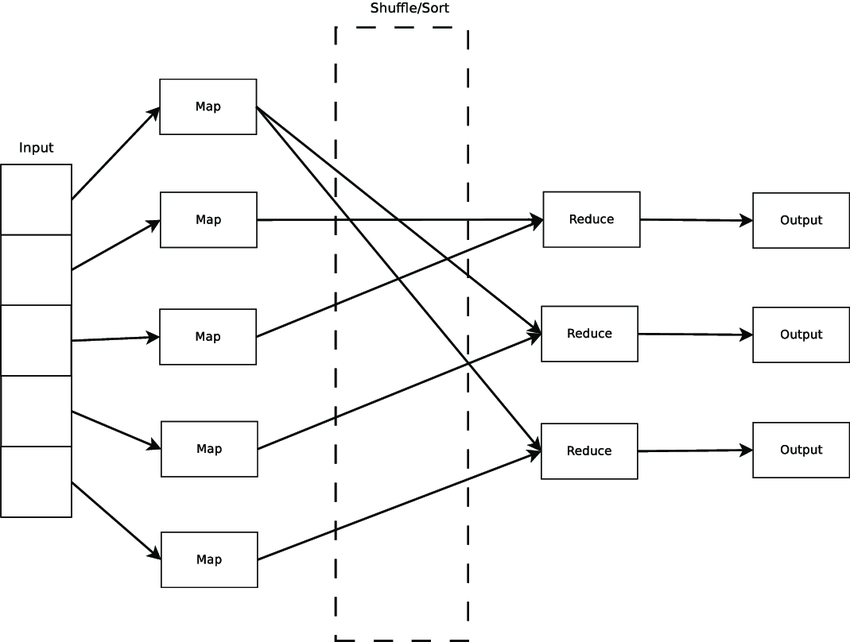
\includegraphics[width=.6\textwidth]{img/mapreduce}
	\caption{\footnotesize Esquema de la arquitectura MapReduce.}
\end{figure}
\end{frame}

\subsection{Diseño e implementación de algoritmos}

%\begin{frame}{Algoritmos difusos de aprendizaje}
%  Se clasifican principalmente en tres tipos:

%  \begin{itemize}
%    \item Basados en \textbf{particiones}. Crean una partición difusa del espacio para medir cómo encajan en ellas los datos y construir reglas en consecuencia.
%    \item \textbf{Neurodifusos}. A partir de una estructura inicial de reglas se emplean modelos neuronales para \textit{ajustar} los parámetros de las funciones de pertenencia.
%    \item \textbf{Genéticos}. Similares a los anteriores, pero se emplean algoritmos genéticos para la fase del ajuste.
%  \end{itemize}
%\end{frame}

\begin{frame}{Algoritmo de Wang y Mendel}
  Propuesto por Wang y Mendel en 1992 para construcción de reglas a partir de datos.

  \begin{enumerate}
    \item Dividir el espacio de entrada en segmentos difusos.
    \item Calcular la pertenencia de cada punto a todas las regiones, y quedarnos en cada caso con las de máxima pertenencia. Así formamos una regla difusa.
    \item Calculamos un peso o \textit{importancia} para cada regla: el producto de la pertenencia del punto a todas las regiones.
    \item Simplificamos la base de datos eliminando duplicados y conflictos eligiendo siempre las reglas de mayor importancia.
    \item Para la predicción, utilizamos el método de defuzzificación COA. Estamos resolviendo un problema de regresión.
  \end{enumerate}
\end{frame}



\begin{frame}[fragile]{Implementación del algoritmo WM}
  \textbf{Etapa map}. Para cada punto calculamos la regla asociada y su importancia.

  \textbf{Etapa reduce}. Agregamos todas las reglas, eliminando conflictos y duplicados.

  \vspace{1em}

  \begin{lstlisting}
val ruleBase = data.mapPartitions { case (x, y) =>
  val (ri, ro, degreeIn, degreeOut)
    = maxRegion(x, y, regionsIn, regionsOut)

  (ri, (ro, degreeIn * degreeOut))
}.reduceByKey { case (r1, r2) =>
  if (r1._2 > r2._2) r1 else r2
}.map { case (ri, (ro, _)) => (ri, ro) }
  \end{lstlisting}
\end{frame}


\begin{frame}{Algoritmo subtractive clustering}
  Propuesto por S. Chiu en 1994 para encontrar número y valor incial de centroides en clústering difuso.

  \textbf{Idea}: cada punto es un posible centroide, y buscamos centroides suficientemente separados. Se asigna inicialmente a cada punto un potencial inversamente proporcional a la distancia a todos los demás.

  \pause
  \begin{enumerate}
    \item Se inicializa el potencial de cada punto y se elige aquel con mayor potencial como centroide.
    \item Se recalculan los potenciales, que disminuyen de forma proporcional a la distancia al centroide elegido.
    \item Se repite el proceso hasta que el potencial cae por debajo de un umbral.
  \end{enumerate}
\end{frame}

\begin{frame}{Versiones del algoritmo subtractive clustering}
  \begin{enumerate}
    \item Verisón \textbf{global}. Para inicializar el potencial se consideran todos los puntos, creando todas las posibles parejas.
    \item Versión \textbf{local}. Se distribuyen los puntos en particiones y el algoritmo se aplica localmente. Después se concatenan los resultados.
    \item Versión \textbf{híbrida}. Se aplica la versión local, se crean grupos de particiones y en ellos se aplica la versión global, utilizando los centroides como datos de entrada.
  \end{enumerate}

  \pause

  Extensión a regresión: cada centroide es una regla difusa. Utilizamos defuzzificación COA.

  Extensión a clasificación: asignar a cada punto la etiqueta del clúster con mayor pertenencia.
\end{frame}

\begin{frame}{Algoritmo Fuzzy C-Means}
  Propuesto por J. Dunn en 1973 y mejorado por J. Bezdek en 1981, para realizar clústering difuso.

  El $i$-ésimo punto tendrá una pertenencia al $j$-ésimo clúster, digamos $u_{ij}$. Se pretende optimizar la función
  \[
    J_m = \sum_{X}\sum_{V} u_{ij}^m\Vert x_i - v_j \Vert^2,
  \]
  sujeta a las restricciones
  \[
    u_{ij}>0 \ \ \forall i, j, \quad y \quad \sum_{V}u_{ij} =1 \ \ \forall i.
  \]
  Se resuelve utilizando los multiplicadores de Lagrange para obtener unas reglas iterativas de actualización de la matriz de pertenencias y los centroides.
\end{frame}

\begin{frame}{Implementación del algoritmo FCM}
  \[
u_{ij}= \dfrac{1}{\displaystyle \sum_{k=1}^c \left( \frac{\Vert x_i - v_j \Vert}{\Vert x_i - v_k \Vert} \right)^{\frac{2}{m-1}}}, \quad \quad \quad v_j = \dfrac{\displaystyle\sum_{i=1}^n u_{ij}^m x_i}{\displaystyle\sum_{i=1}^n u_{ij}^m}.
  \]
  \vspace{.5em}

  \textbf{Etapa map}. Se calculan para cada punto los valores necesarios para actualizar los centroides. No se mantiene en memoria la matriz de pertenencia.

  \textbf{Etapa reduce}. Para cada centroide, se suman entre sí los valores obtenidos en la etapa anterior.

  Extensión a clasificación: procedemos como en el algoritmo anterior. En este caso se asigna a cada clúster la etiqueta de la clase mayoritaria tras un conveniente $\alpha$-corte.
\end{frame}

\subsection{Estudio comparativo}

\begin{frame}{Comparación de precisión en clasificación}
  \begin{figure}
	\centering
	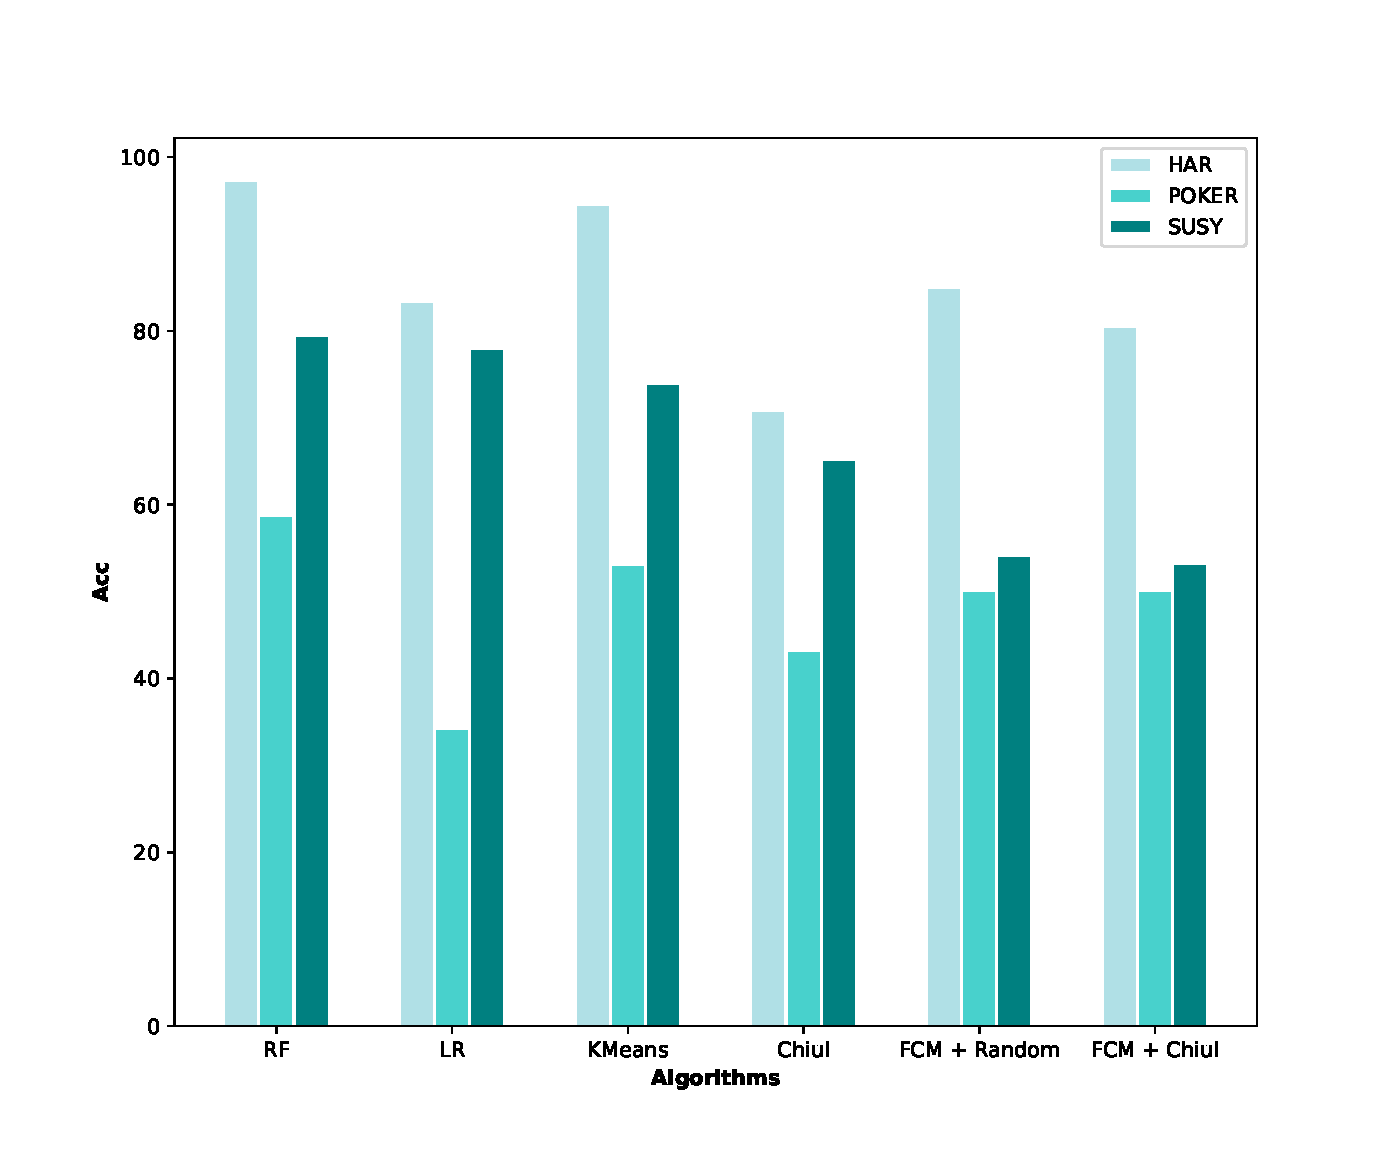
\includegraphics[width=.75\textwidth]{img/acc-class}
	\caption{\footnotesize Comparación de la precisión obtenida en los tres conjuntos de datos elegidos para los algoritmos de clasificación.}
\end{figure}
\end{frame}

\begin{frame}{Comparación de tiempo en clasificación}
  \begin{figure}
	\centering
	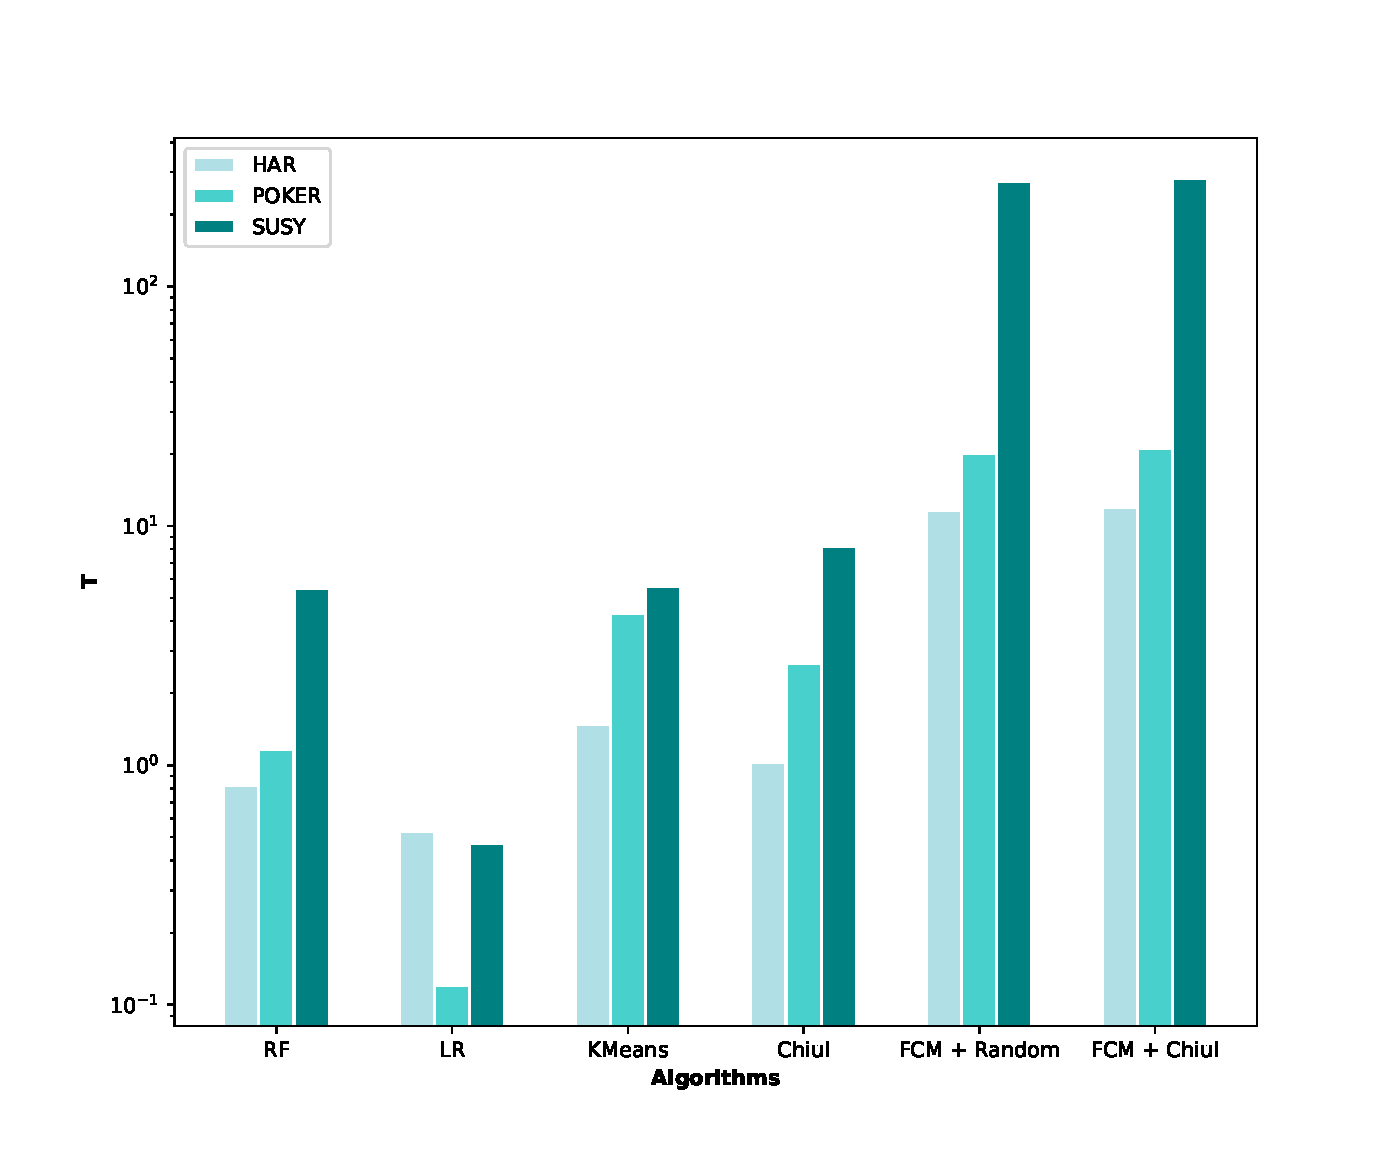
\includegraphics[width=.75\textwidth]{img/time-class}
	\caption{\footnotesize Comparación del tiempo de ejecución en los tres conjuntos de datos elegidos para los algoritmos de clasificación.}
\end{figure}
\end{frame}

\begin{frame}{Comparación de error en regresión}
    \begin{figure}
	\centering
	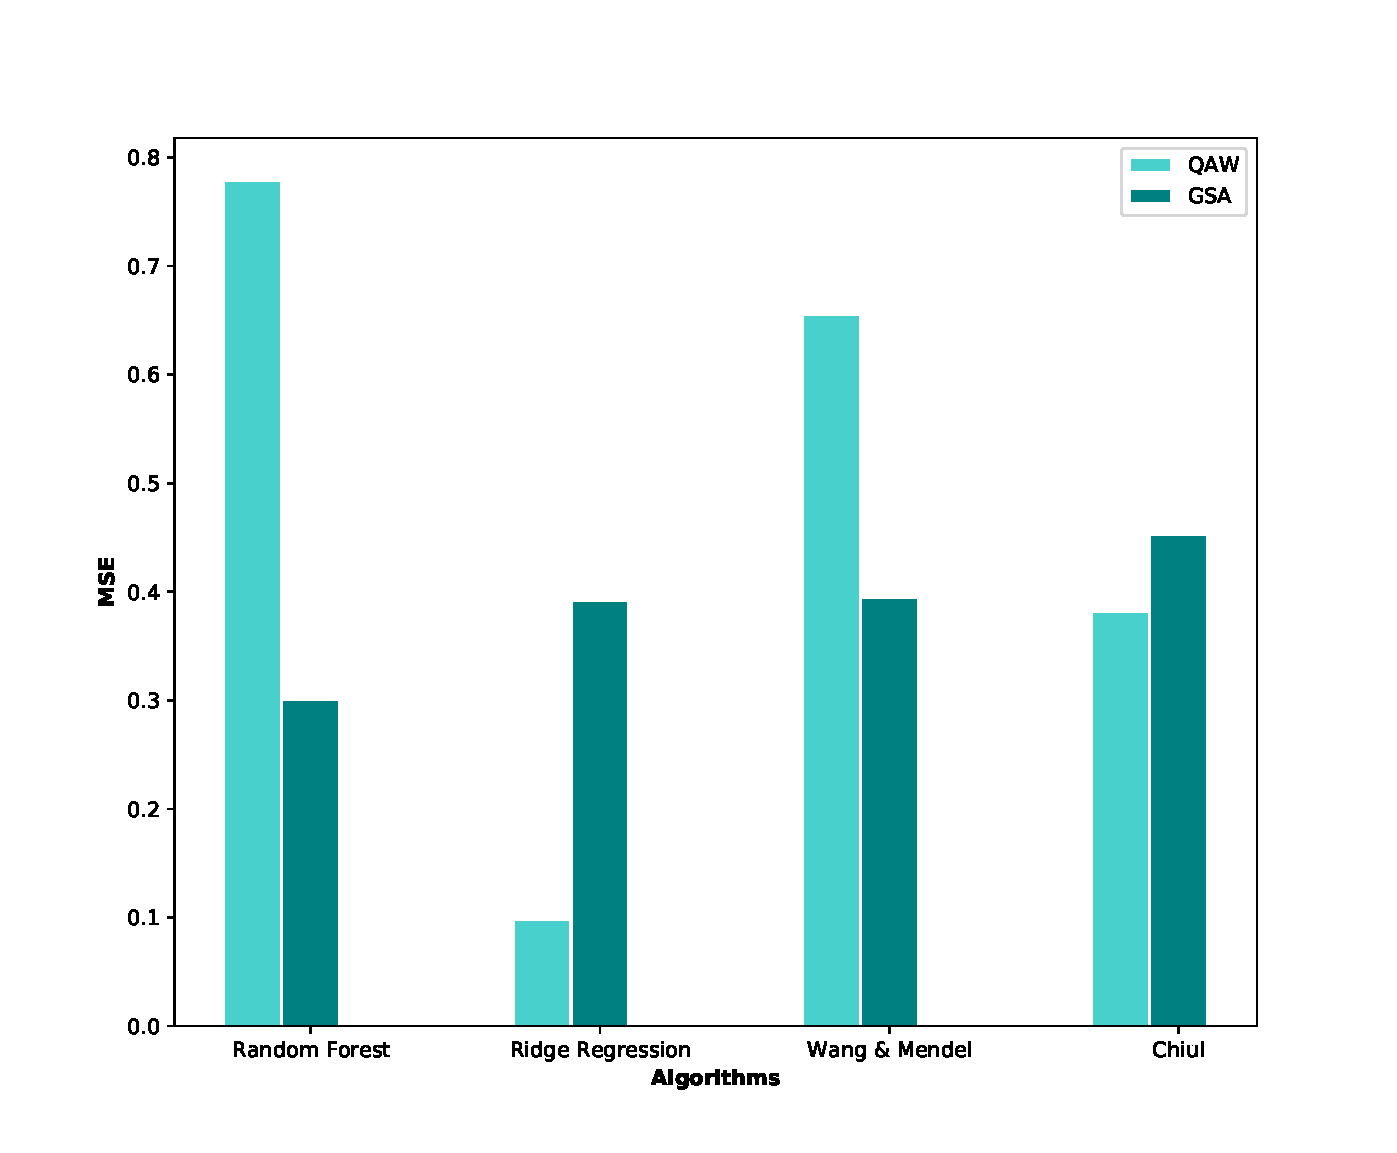
\includegraphics[width=.75\textwidth]{img/mse-reg}
	\caption{\footnotesize Comparación del Mean Squared Error en los dos conjuntos de datos elegidos para los algoritmos de regresión.}
\end{figure}
\end{frame}

\begin{frame}{Comparación de tiempo en regresión}
  \begin{figure}
	\centering
	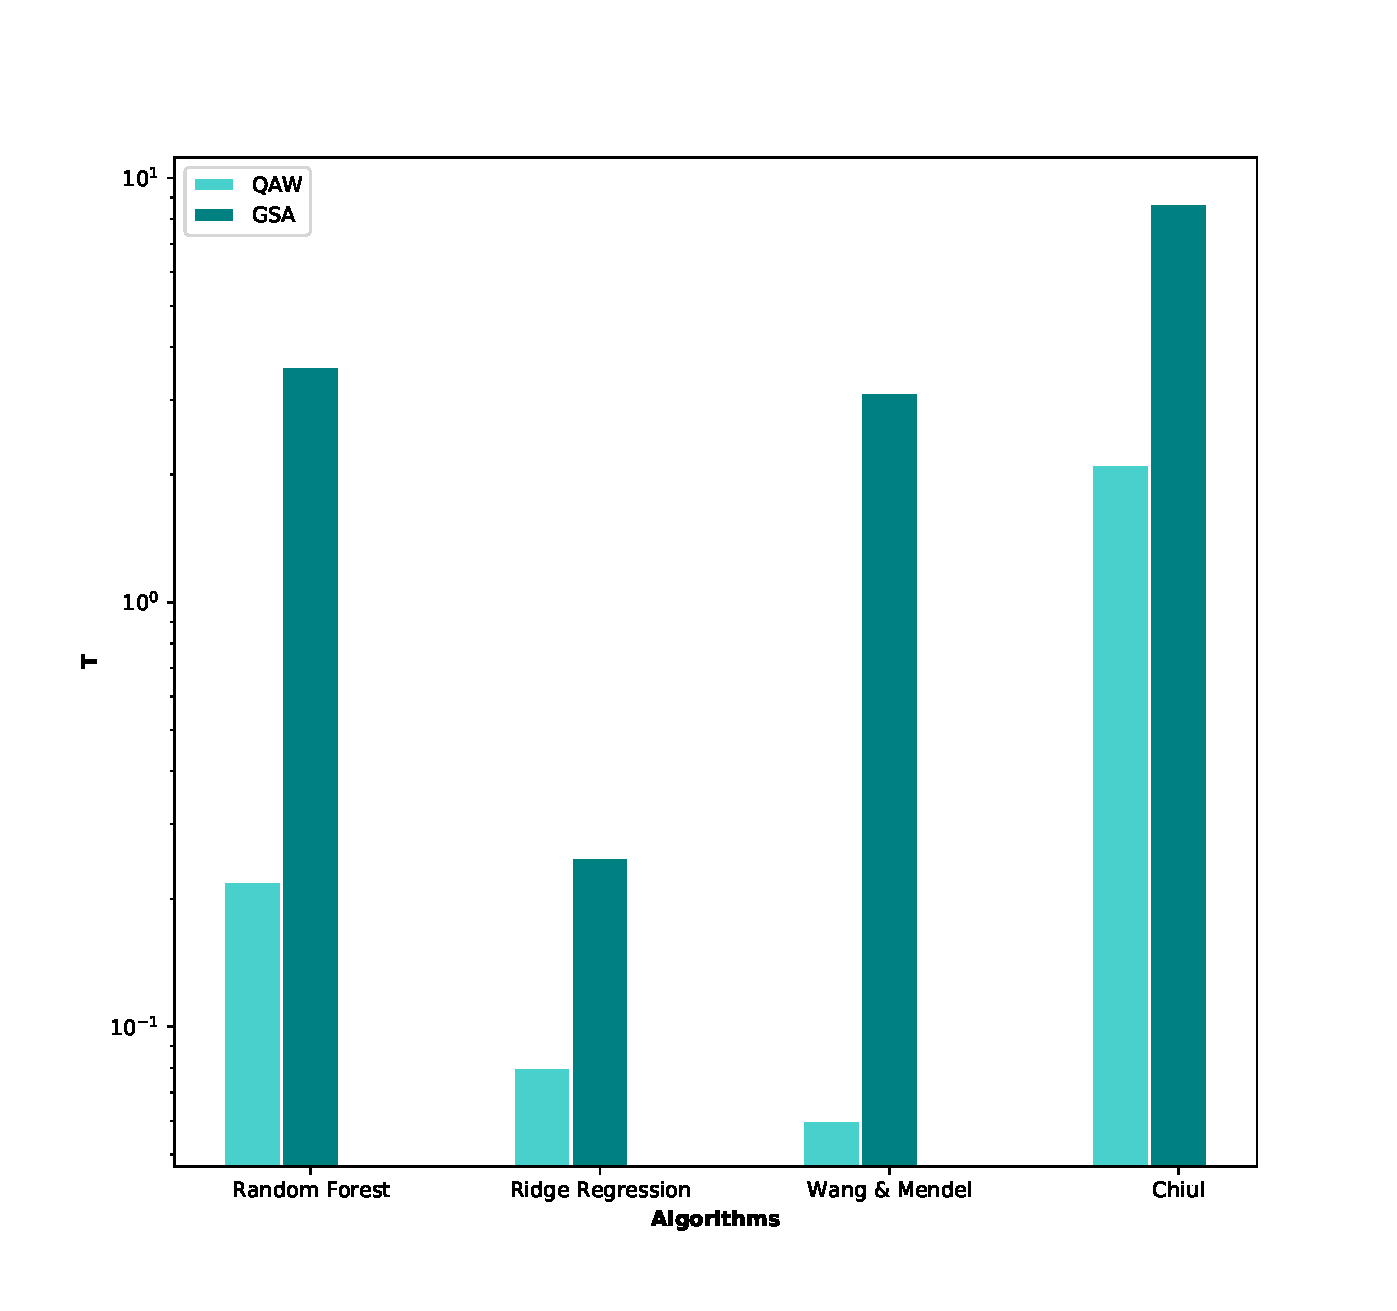
\includegraphics[width=.65\textwidth]{img/time-reg}
	\caption{\footnotesize Comparación del tiempo de ejecución en los dos conjuntos de datos elegidos para los algoritmos de regresión.}
\end{figure}
\end{frame}

\begin{frame}{Conclusiones}
    \begin{itemize}[<+->]
      \item Hemos realizado una aportación original desarrollando algoritmos escalables para aprendizaje de sistemas difusos, justificando su interés teórico y práctico.
      \item Hemos comprobado que es necesario un diseño cuidadoso para adaptar los algoritmos al escenario Big Data. No basta una mera paralelización.
      \item Nos hemos familiarizado con el modelo de referencia MapReduce y las herramientas del estado del arte en el Big Data, como Apache Spark y HDFS.
    \end{itemize}
\end{frame}

\begin{frame}{Referencias}
\begin{thebibliography}{9}

\bibitem{neuro-fuzzy}
  \textsc{Jang, J. S. R., Sun, C. T., \& Mizutani, E}. \textit{Neuro-fuzzy and soft computing; a computational approach to learning and machine intelligence}. (1997).

\bibitem{wm}
\textsc{L.X. Wang, J. M. Mendel}. \textit{Generating fuzzy rules by learning from examples.} (1992).

\bibitem{chiu}
\textsc{S. Chiu}. \textit{Fuzzy Model Identification Based on Cluster Estimation.} (1994).

\bibitem{wm}
\textsc{James C. Bezdek \textit{et al}}. \textit{Detection and Characterization of Cluster Substructure I. Linear Structure: Fuzzy c-Lines.} (1981).


\end{thebibliography}
\end{frame}

\section{Ecuaciones no resolubles con respecto a la derivada}

%\begin{frame}{Notas finales}
%	Estas diapositivas, junto con unas notas algo más detalladas sobre conjuntos y lógica difusa (en inglés), pueden descargarse en:
%\begin{center}
%\href{https://github.com/antcc/fuzzy-systems}{\url{github.com/antcc/fuzzy-systems}}
%\end{center}

%{%
%\metroset{block=transparent}
%\begin{alertblock}{Nota.}
%\vspace{.005em}
%Todas las imágenes y figuras, salvo que se especifique lo contrario, han sido extraídas de \cite{neuro-fuzzy}.
%\end{alertblock}
%}
%\end{frame}


\begin{frame}[standout]
Gracias por su atención
\end{frame}

\end{document}
